\documentclass[a4paper,10pt]{article}
\usepackage[utf8]{inputenc}
\usepackage[T1]{fontenc}
%\usepackage{geometry}
\usepackage{graphicx}

\begin{document}

\begin{center}
% Title
{\Large \bf Exact results for electronic eigenstates in one and two dimensional quasicrystals.}
\vspace{1cm}

% Authors
Nicolas Macé, Anuradha Jagannathan, Frédéric Piéchon $^1$, Rémy Mosseri$^2$

\vspace{0.5cm}
% Affiliations
{\it $^1$ Laboratoire de Physique des Solides, Univ. Paris-Sud, Université Paris-Saclay, 91400 Orsay, France}

{\it $^2$ Laboratoire de Physique Théorique de la Matière Condensée, Université Pierre et Marie Curie, Place Jussieu, 75252 Paris, France}

\end{center}

\vspace{0cm}

% Abstract

Single-electron properties of 1D quasicrystals are well understood: the spectrum of quasiperiodic chains can be described exactly for a number of tight-binding models [1], and the wavefunctions are also rather well characterized [2].
In contrast, even the simplest models of 2 and 3 dimensional quasicrystals resist theoretical investigations.
The spectrum and corresponding wavefunctions of a simple tight-binding model on the Penrose lattice, for instance, were only known approximately, by numerical computations, until recently.

This situations changed recently when Kalugin and Katz [3] proposed an analytical form for the ground state of two dimensional quasiperiodic tight-binding models and showed that it fitted numerical results on the Penrose and Ammann-Beenker tilings (see figure for Penrose).
We show that simpler one-dimensional versions of this ansatz exist generally for hopping models on a family of aperiodic chains including the Fibonacci chain.
We show how these ``critical'' states depend on the geometric properties of the tilings and compute explicitly the multifractal properties of these states. 
Similar calculations are shown to be possible for the two dimensional case, for a family of Hamiltonians.
Analytical expressions for the transport characteristics are presented for the 1D case. 


% Si vous voulez inclure une figure, decommentez les 4 lignes ci-dessous, et
% envoyez l'ensemble (.tex+figure) sous forme d'une archive .zip ou .tar.gz

\vspace{0cm}
\begin{center}
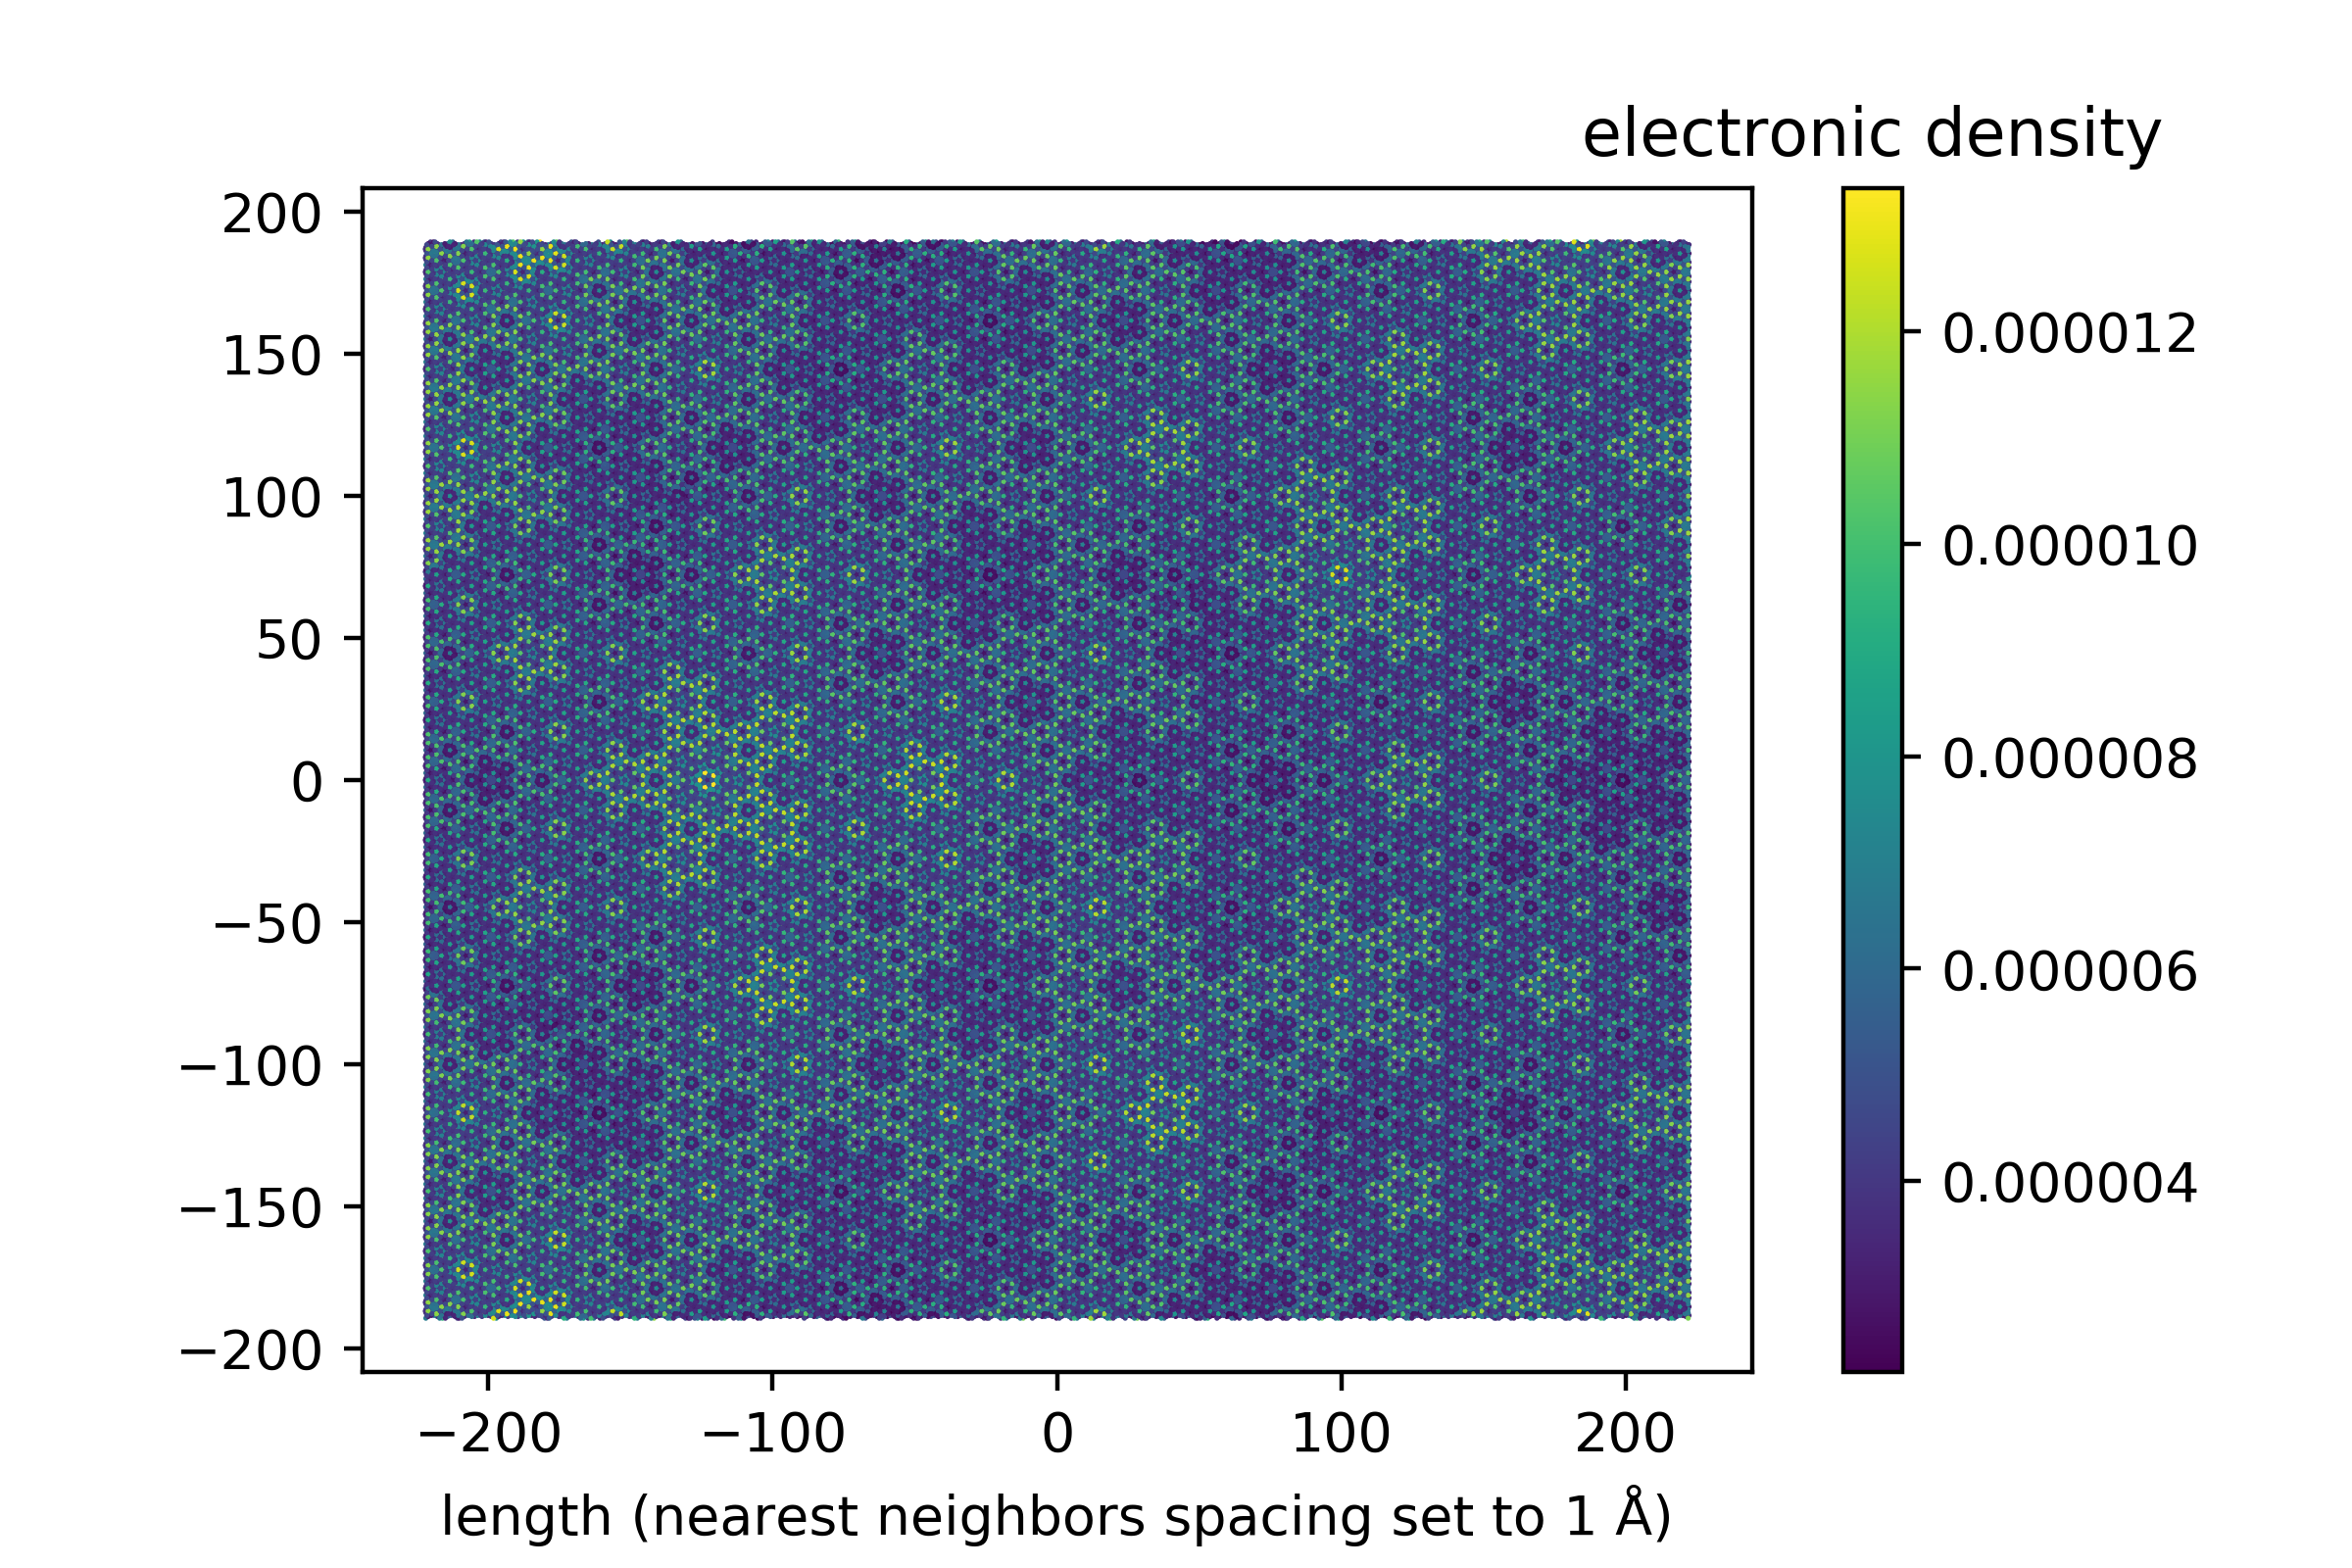
\includegraphics[width=0.9\textwidth]{taylor_9_groundstate.png}
\end{center}
%\textwidth
[1] A. Rüdinger, C. Sire, J Phys A, 1996. 
[2] N. Macé, A. Jagannathan, F. Piéchon, Phys Rev B, 2016.
[3] P. Kalugin, A. Katz, J Phys A, 2014.
[4] N. Macé, A. Jagannathan, F. Piéchon, R. Mosseri, In preparation, 2017.
\end{document}
